\begin{tikzpicture}
	%axis
	\begin{scope} [decoration={border, segment length=1cm, amplitude=1mm, angle=90}]
		\draw[postaction={decorate, draw}] (-5, 0) -- (5.1, 0);
		\draw[postaction={decorate, draw}] (0, 0) -- (0, 5.1); 
	\end{scope}
	
	\def\lzero{(-5, 1) cos (-2.5, 1.5) sin (0,2) cos (2.5, 1.5) sin (5, 1)};
	\fill[cyan, opacity=0.2] \lzero;
	\draw[cyan!75!black] \lzero node[right, black] {$\Psi_0(x)$};
	
	\def\lone{(-5, 2.5) cos (-3.33, 2.25) sin (-1.66, 2) cos (0, 2.5) sin (1.66, 3) cos (3.33, 2.75) sin (5, 2.5)}
	\fill[red, opacity=0.2] \lone;
	\draw[red!75!black] \lone node[right, black] {$\Psi_1(x)$};
	
	\def\ltwo{(-5, 4) cos (-3.75, 4.25) sin (-2.5, 4.5) cos (-1.25, 4) sin (0, 3.5) cos (1.25, 4) sin (2.5, 4.5) cos (3.75, 4.25) sin (5, 4)}
	\fill[green, opacity=0.2] \ltwo;
	\draw[green!75!black] \ltwo node[right, black] {$\Psi_2(x)$};
	
	\draw (0, 0) parabola (5, 5);
	\draw (0, 0) parabola (-5, 5);
	
	\draw[latex-latex, red] (-5, -1.5) -- (5, -1.5);
	\node[above, red] at (0, -1.5) {$T = \dfrac{2 \pi}{\omega_f}$ von $f$};
	
	\draw[dashed, red] (-5, -1.5) -- (-5, 5);
	\draw[dashed, red] (5, -1.5) -- (5, 5);
\end{tikzpicture}